The Beneš network is an extension of the Banyan network.
It solves the problem that a Banyan network is not able to produce all possible permutations by mirroring the Banyan network and connecting the two.
An example for a Beneš network with 8 inputs is given in Figure \ref{fig:benes}.

The two halves of the network are different in the routing procedure employed.
For the output half, the destination of a data packet defines the exact setting of every switch on its path, because there always is only one possible choice.
The input half is responsible for conflict avoidance, which has a significantly higher complexity due to the fact that it depends on all inputs of one column of the network.

For implementation, the recursive structure given in Figure \ref{fig:benes_recursion} was used.
A network with $2^n$ inputs is defined as $benes(n, n)$, where the first parameter gives the size of the specific network defined, and the second is used during recursion to remember the size of the whole network.

For this structure, the routing decision of the output switches is based on just bit $k - 1$, where a $0$ requires the packet to go up and $1$ to go down.

\begin{figure}[!ht]
	\centering
	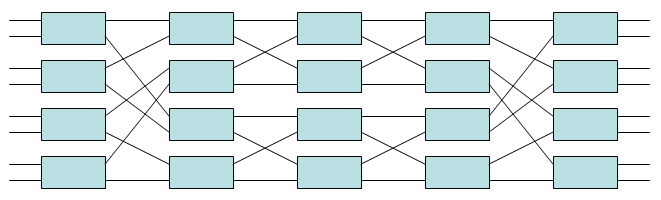
\includegraphics[width=\linewidth]{Benesnetwork.png}
	\caption{
		The basic structure of a Benes Network \\
		(source: https://commons.wikimedia.org/wiki/File:Benesnetwork.png)
	}
	\label{fig:benes}
\end{figure}


\begin{figure}[!ht]
	\centering
	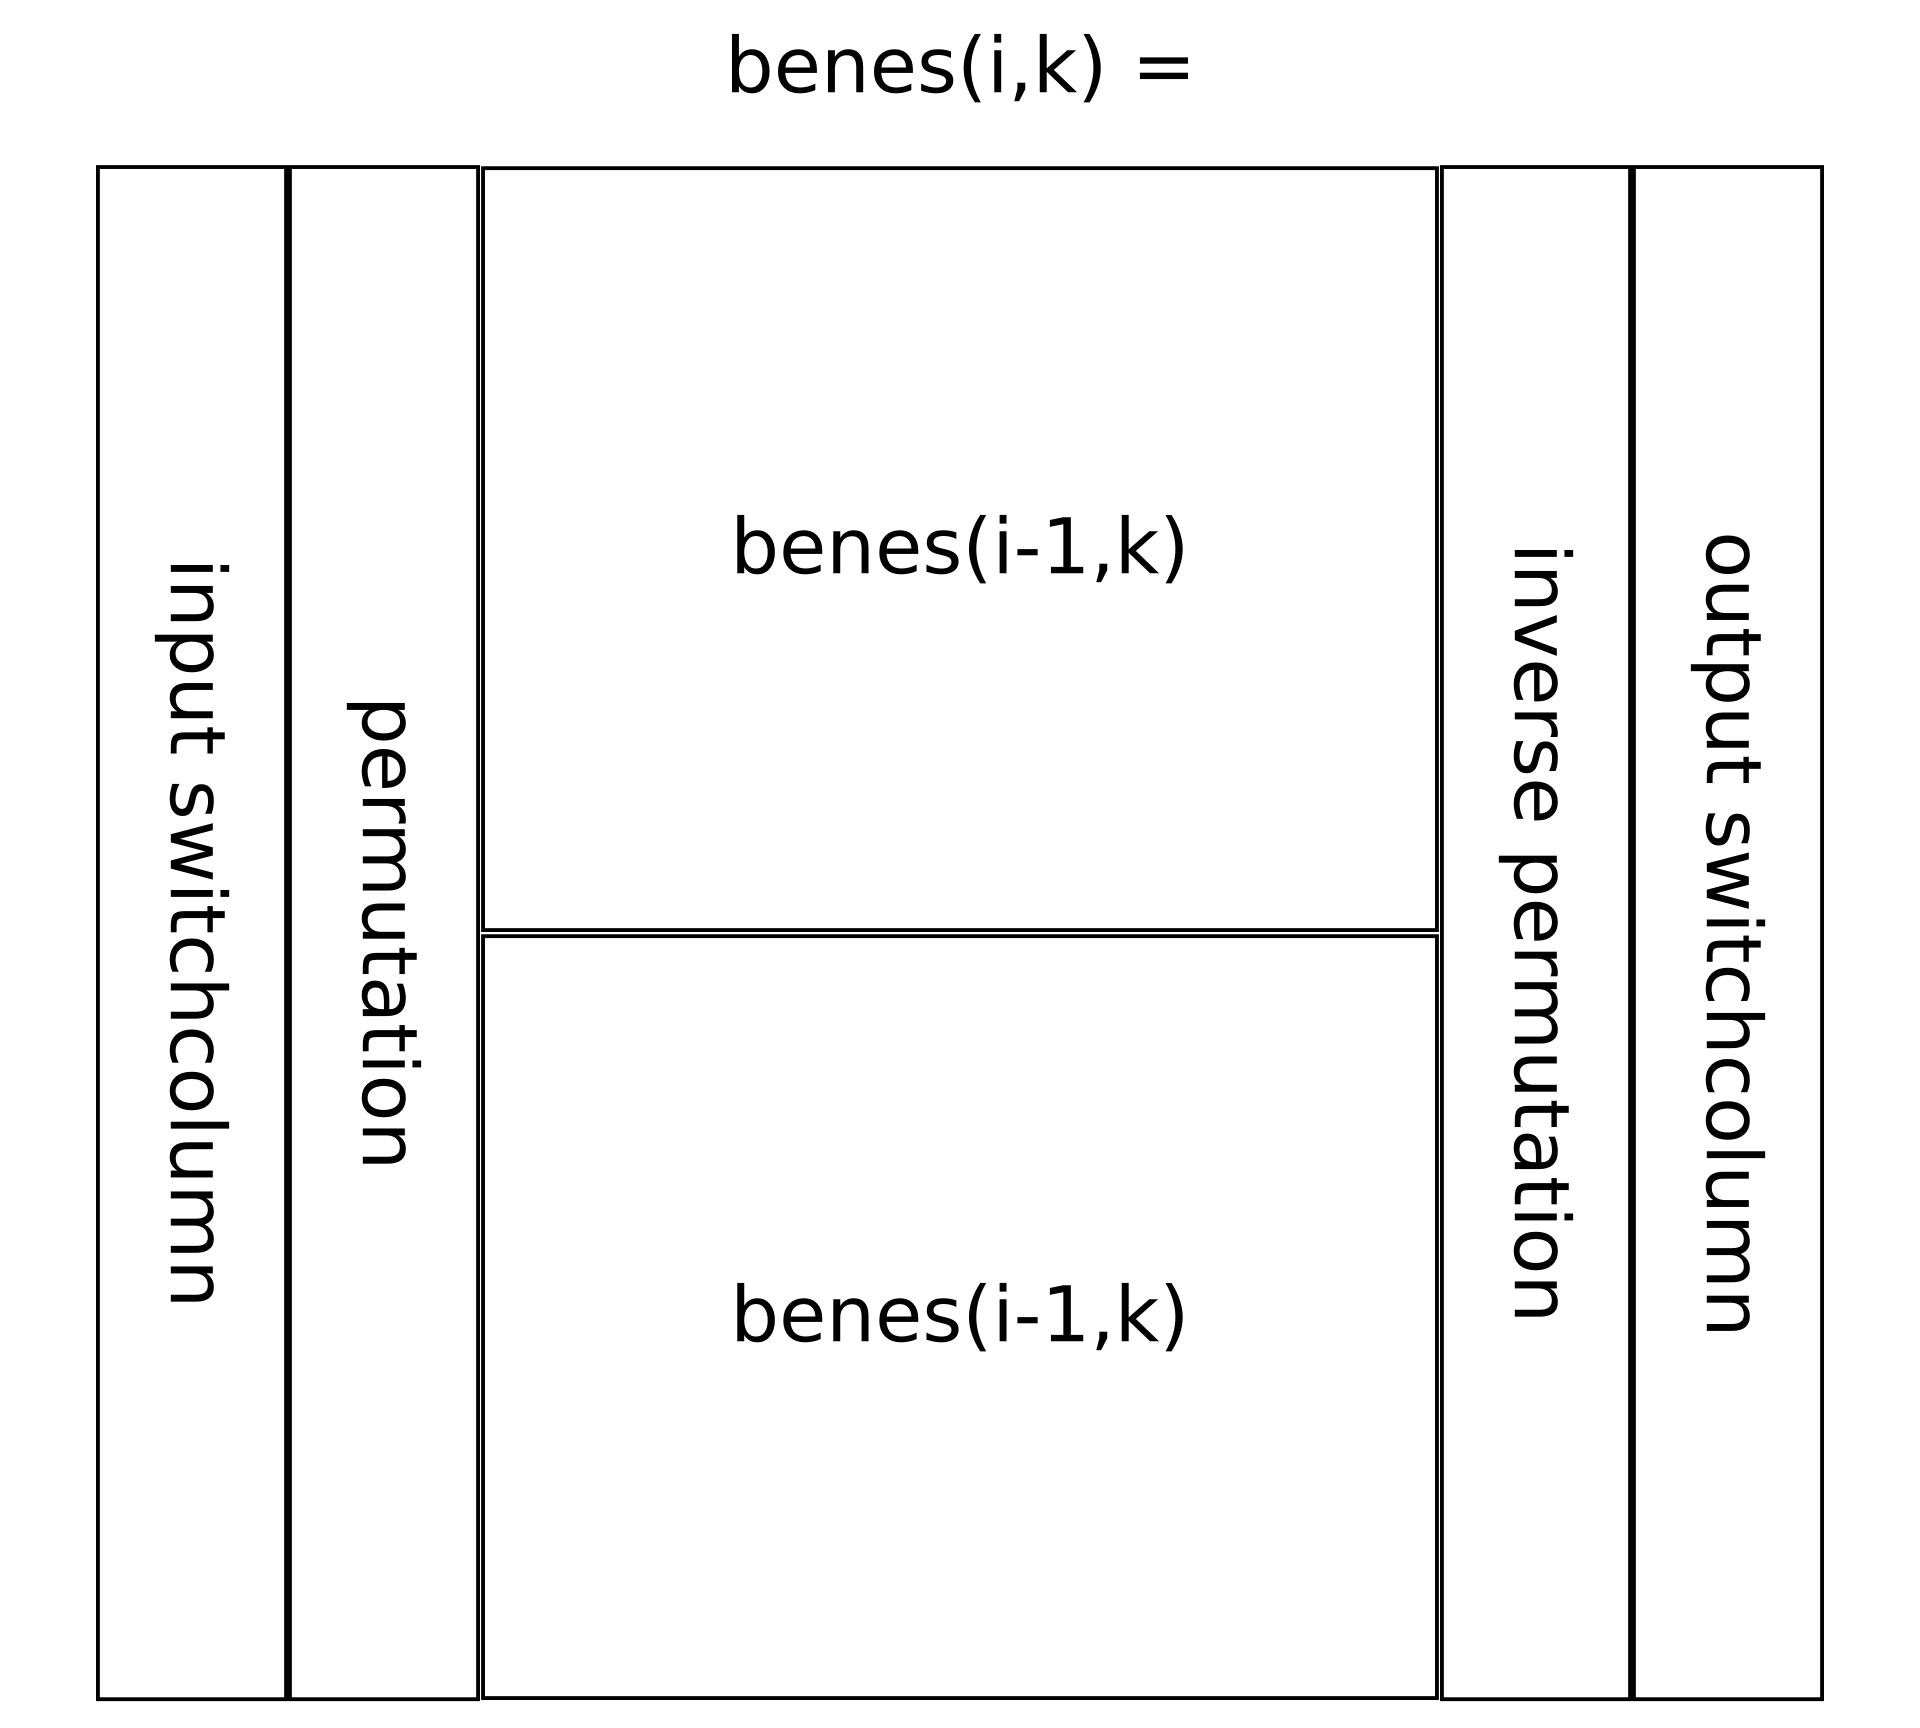
\includegraphics[width=\linewidth/2]{benes_recursion.png}
	\caption{recursive definition of a benes network}
	\label{fig:benes_recursion}
\end{figure}

